\documentclass[conference]{IMSTemplate}

\usepackage{amsmath}
\usepackage{amssymb}
\usepackage{graphicx}
\usepackage{booktabs}
\usepackage{array}
\usepackage{url}
\usepackage{cite}

\graphicspath{{./}{docs/}}

\title{Acceleration of One-Head Transformer Attention on a Xilinx Alveo U55C FPGA}

\author{Samarth Bangalore Sudharshan, Rijul Wankhade, Om Girish Sheladia, and
Satyarth Guna Motupalli\\
CEN571: Reconfigurable Computing\\
Arizona State University}

\begin{document}

\maketitle

\begin{abstract}
Transformer inference is increasingly important for edge and local deployment,
but attention layers remain expensive because their score matrix grows
quadratically with sequence length. This work implements and evaluates a
specialized FPGA data path for accelerating the core attention computation used
by a TinyLlama-derived model. The implemented system targets a Xilinx Alveo
U55C and offloads one attention head, beginning from RoPE-rotated
integer-quantized query and key tensors and a floating-point value tensor. The
verified hardware path computes INT8 query-key scores, applies causal masking
and dequantization scaling, performs full-row softmax, and computes
\(\mathrm{softmax}(QK^T)V\) to produce a one-head floating-point attention
output. The design is intentionally narrower than full TinyLlama inference: it
does not implement Q/K/V projection, RoPE generation, decoder integration, or
model-level token generation. The final fused design passes local C++ checks,
Vitis HLS C simulation and synthesis, XRT hardware emulation, and real U55C
execution for synthetic sequence lengths \(S=8,64,128,256,512\) and
TinyLlama-derived vector directories at \(S=16,64,128,256,512\). On real
hardware, the fused FPGA path runs the synthetic \(S=512\) one-head attention
case in 60.328 ms and the real TinyLlama-derived \(S=512\) vector case in
55.329 ms. The synthetic \(S=512\) CPU NumPy baseline is 12.329 ms, and the RTX
3050 Laptop GPU PyTorch baseline is 0.246 ms. These results show a correct and
verified FPGA attention block with clean post-route timing closure, but also
show that the current staged architecture is dominated by repeated kernel
launches and host-visible HBM staging. The work establishes a validated
baseline and identifies the next architectural improvements: device-resident
data flow, reduced launch count, online softmax fused with value accumulation,
and parallel execution across query blocks or heads.
\end{abstract}

\noindent\textbf{Keywords---}FPGA, transformer attention, TinyLlama, Xilinx
Alveo U55C, HLS, XRT, HBM, softmax, quantization.

\section{Introduction}

Large language models are moving from cloud-only services toward local and edge
deployments, where privacy, availability, and latency constraints make remote
execution less attractive. Edge LLM systems must process user prompts locally,
respond within a tight latency budget, and operate under more limited power and
thermal envelopes than data-center GPUs. These requirements motivate hardware
acceleration techniques that can exploit the structure of transformer
computation rather than relying only on general-purpose processors.

The attention mechanism is one of the defining operations in transformer
models. For a sequence of \(S\) tokens, each attention head computes a score
matrix \(QK^T\), applies a causal mask and scaling, converts each score row to
probabilities with softmax, and uses those probabilities to form a weighted sum
of values. Even for one head, the score matrix is \(S \times S\), so storage
and compute grow quickly as the sequence length increases. In a full model such
as TinyLlama, this operation is repeated across multiple layers and multiple
attention heads. This regular structure makes attention a natural candidate for
FPGA acceleration, especially when combined with low-precision arithmetic,
tiling, on-chip buffering, and high-bandwidth memory.

This work studies the FPGA offload of a focused attention block rather than
a full language model. The goal is to understand what is required to map
TinyLlama-style attention onto the Xilinx Alveo U55C, verify the result on real
hardware, and measure where the first implementation succeeds or falls short.
The selected hardware boundary begins after the model has computed
RoPE-rotated query and key tensors and a value tensor. Query and key are
quantized to INT8 with per-tensor scale factors, while value and final
attention output remain FP32. The FPGA computes the one-head attention result:
\[
    \mathrm{attn\_out} =
    \mathrm{softmax}\left(\frac{QK^T}{\sqrt{d_h}} + M\right)V,
\]
where \(d_h=64\) is the head dimension and \(M\) is the causal mask.

The work evolved through four tracks. Track A made the attention
score pipeline work across real sequence lengths using tiling, full-row
softmax, double buffering for the pre-softmax pass, and finally a fused
score-mask-scale kernel. Track B added the value weighted-sum stage so the FPGA
produces final one-head attention output rather than only attention
probabilities. Track C replaced purely synthetic inputs with TinyLlama-derived
Q/K/V vectors. Track D collected CPU, GPU, FPGA, timing, utilization, and
verification results. The resulting design is a correct one-head attention
accelerator, not a complete TinyLlama runtime. This distinction matters because
the reported times are attention-block latencies, not generated-token
throughput.

The main contribution is therefore twofold. First, it provides a
complete verified U55C implementation of a tiled one-head attention path,
including Python reference generation, HLS kernels, XRT host orchestration, HBM
bank placement, hardware emulation, real-card validation, and post-route
reports. Second, it exposes the architectural bottleneck in a straightforward
staged implementation: although the FPGA kernels are correct and timing closes,
the system remains slower than CPU and GPU baselines because it launches many
small kernels and materializes intermediates in host-visible HBM buffers.

\section{Background and Prior Work}

\subsection{Edge LLM Motivation}

Running language models near the user has different requirements from running
them in a centralized GPU cluster. A local assistant, industrial controller, or
embedded analysis system may need to keep prompts private, continue operating
when a network connection is unavailable, and stay within a fixed power budget.
At the same time, the system must still perform the transformer operations that
dominate modern language models. The result is a hardware problem: the
accelerator must provide enough throughput and low enough latency without the
thermal and cost assumptions of a large server GPU.

FPGAs are attractive in this setting because they can be specialized after
deployment. If a model uses fixed head dimensions, fixed quantization formats,
or a known maximum sequence length, an FPGA design can harden those choices
into a dedicated datapath with custom arithmetic width, explicit memory banking,
and fine-grained loop parallelism that general-purpose processors cannot expose.
However, these benefits only appear when the design is architecturally matched
to the workload. A naive staged FPGA implementation can
easily lose to software if the host must launch hundreds or thousands of small
kernels and move intermediate matrices through external memory after every
stage. This work demonstrates both sides of that tradeoff: a correct FPGA attention
block was built and verified, but the first staged implementation is not yet
competitive with software for this isolated workload.

\subsection{Transformer Attention}

The transformer architecture introduced self-attention as a replacement for
recurrent sequence processing \cite{alammar2018illustrated,leo2024math}. In a causal decoder
model, each token is allowed to attend only to itself and previous tokens. For
one attention head, the input representation is projected into query, key, and
value matrices:
\[
    Q, K, V \in \mathbb{R}^{S \times d_h}.
\]
The unnormalized attention scores are:
\[
    L = QK^T,
\]
where \(L \in \mathbb{R}^{S \times S}\). The scaled and masked logits are:
\[
    \hat{L}_{ij} =
    \begin{cases}
    L_{ij}/\sqrt{d_h}, & j \leq i,\\
    -\infty, & j > i.
    \end{cases}
\]
Softmax is applied independently to each row:
\[
    P_{ij} = \frac{e^{\hat{L}_{ij} - m_i}}
                  {\sum_{k=0}^{S-1} e^{\hat{L}_{ik} - m_i}},
    \quad
    m_i = \max_j \hat{L}_{ij}.
\]
Finally, attention output is:
\[
    O = PV.
\]
The subtraction of \(m_i\) is the standard numerically stable softmax form
\cite{nielsen2015neural,alammar2018illustrated,leo2024math}.

TinyLlama uses hidden dimension 2048 and 32 query heads, giving a head
dimension of 64. This work focuses on one selected head. TinyLlama also uses
grouped-query attention with fewer key/value heads than query heads; the
extraction flow maps the selected query head to the corresponding key/value
group before exporting vectors for FPGA verification.

\subsection{FPGA Suitability}

FPGAs are well suited to regular, streaming, and tiled data paths. They allow
custom arithmetic width, explicit memory banking, loop pipelining, and
fine-grained parallelism. For attention, the \(QK^T\) stage is a dense dot
product over a fixed head dimension, while the \(PV\) stage is another matrix
product over the sequence axis. Both operations can be tiled to fit local
buffers and mapped to DSP-heavy datapaths.

The Alveo U55C provides HBM, multiple SLRs, and a Vitis/XRT software stack for
kernel compilation and host control. In this design,
XRT is responsible for loading the xclbin, allocating buffer objects,
syncing data between host and device, launching kernels, and reading back
results. Vitis HLS is used to compile C++ HLS top functions into FPGA kernels.

\subsection{Prior Acceleration Approaches}

Prior work on neural network acceleration often focuses on reducing precision,
reusing on-chip data, and fusing operations to avoid external memory traffic.
Transformer accelerators additionally try to avoid materializing the full
attention probability matrix, because it requires \(O(S^2)\) storage. Online
softmax algorithms address this by streaming over key/value blocks while
maintaining a row maximum, normalization sum, and value accumulator. This
work's verified baseline does not yet implement online softmax, but it is
identified as the most important future optimization after device-resident
buffers and launch-count reduction.

The design therefore uses a staged methodology rather than jumping directly to
a monolithic online-attention kernel. Each stage is verified first: score
generation, mask and scale, full-row softmax, and value accumulation. The
benefit of this approach is observability---intermediate tensors can be compared
against Python references at each stage. The drawback is that a staged design
materializes intermediate data and exposes more control work to the host. These
results should be interpreted with that tradeoff in mind.

\section{Project Description}

\subsection{Scope}

The implemented system accelerates one attention head from a TinyLlama-derived
path. The input to the FPGA-side computation is:
\[
Q_{\mathrm{int8}}, K_{\mathrm{int8}}, V_{\mathrm{fp32}},
\]
where Q and K already include rotary positional embedding in the exported
software flow. The output is:
\[
O_{\mathrm{fp32}} \in \mathbb{R}^{S \times 64},
\]
the attention output for one head. The design does not produce text, logits
over the vocabulary, or a complete transformer-layer output.

The out-of-scope components are Q/K/V projection GEMMs, RoPE generation, layer
normalization, feed-forward layers, key/value cache management, decoder-layer
integration, and full TinyLlama token generation. Keeping these components out of scope allowed the core matrix operations to be
verified end-to-end while preserving the mathematically important part of
attention.

The design also focuses on prefill-style full-sequence attention rather than
incremental decode with a key/value cache. In a decode workload, each new token
uses one query row and attends over cached keys and values. In the implemented
test cases, the full \(S\times S\) attention pattern is evaluated for a saved
sequence. This is appropriate for validating the core matrix operations and for
comparing synthetic sequence lengths, but a deployed LLM runtime would need
additional logic for cache layout, streaming token inputs, and interaction with
the surrounding decoder layer.

\subsection{Data Types and Quantization}

The query and key tensors are quantized using per-tensor symmetric INT8 scales.
If \(q_s\) and \(k_s\) are the scale factors, the approximate dequantized values
are:
\[
    Q_{\mathrm{fp32}} \approx q_s Q_{\mathrm{int8}},
    \quad
    K_{\mathrm{fp32}} \approx k_s K_{\mathrm{int8}}.
\]
The raw dot product is accumulated in INT32:
\[
    R_{ij} = \sum_{d=0}^{63} Q_{\mathrm{int8}}[i,d]K_{\mathrm{int8}}[j,d].
\]
The fused score-mask-scale kernel then computes:
\[
    \hat{L}_{ij} =
    \begin{cases}
    R_{ij}q_s k_s / 8, & j \leq i,\\
    -10^9 q_s k_s / 8, & j > i,
    \end{cases}
\]
where \(1/\sqrt{64}=1/8\). The implementation uses \(-10^9\) as the raw
finite mask sentinel before scaling rather than literal negative infinity to
keep the kernel simple and deterministic. Softmax, value, and attention output
use FP32 in the verified design.

\subsection{Tiling}

The hardware tile shape is fixed around the head dimension:
\[
\begin{aligned}
Q_{\mathrm{tile}} &: 8 \times 64,\\
K_{\mathrm{tile}} &: 64 \times 64,\\
\mathrm{score}_{\mathrm{tile}} &: 8 \times 64.
\end{aligned}
\]
For sequence length \(S\), the number of score tiles per head is:
\[
    N_{\mathrm{tiles}} =
    \left\lceil \frac{S}{8} \right\rceil
    \left\lceil \frac{S}{64} \right\rceil .
\]
The implementation handles non-full tiles through active row and column counts.
Inactive rows or columns are padded and ignored rather than discarded.
Table~\ref{tab:tilecounts} lists the resulting tile counts for the synthetic
sequence lengths used in the evaluation.

\begin{table}[t]
\centering
\caption{Tile counts for the tested synthetic sequence lengths.}
\label{tab:tilecounts}
\begin{tabular}{rrrr}
\toprule
\(S\) & Q chunks & K chunks & Score tiles \\
\midrule
8   & 1  & 1 & 1 \\
64  & 8  & 1 & 8 \\
128 & 16 & 2 & 32 \\
256 & 32 & 4 & 128 \\
512 & 64 & 8 & 512 \\
\bottomrule
\end{tabular}
\end{table}

For \(S>64\), softmax cannot be applied independently to each \(8\times64\)
score tile. Each query row must be normalized across all \(S\) keys. Therefore,
the host assembles full \(8\times S\) logit rows from all key chunks, launches a
full-row softmax kernel, slices the resulting probability rows into
\(8\times64\) tiles, and passes those tiles to the value weighted-sum kernel.

For example, at \(S=512\), the FPGA processes 64 Q chunks and 8 K chunks per
head. The score stage therefore launches 512 tile computations. Full-row
softmax launches once per Q chunk, for 64 more launches. The V weighted-sum
stage launches once per Q/K chunk, adding another 512 launches. This yields
1088 kernel launches for one head. That launch count is the dominant performance bottleneck.
Figure~\ref{fig:architecture} summarizes the final fused one-head datapath and
the host-visible HBM buffers.

\begin{figure*}[t]
    \centering
    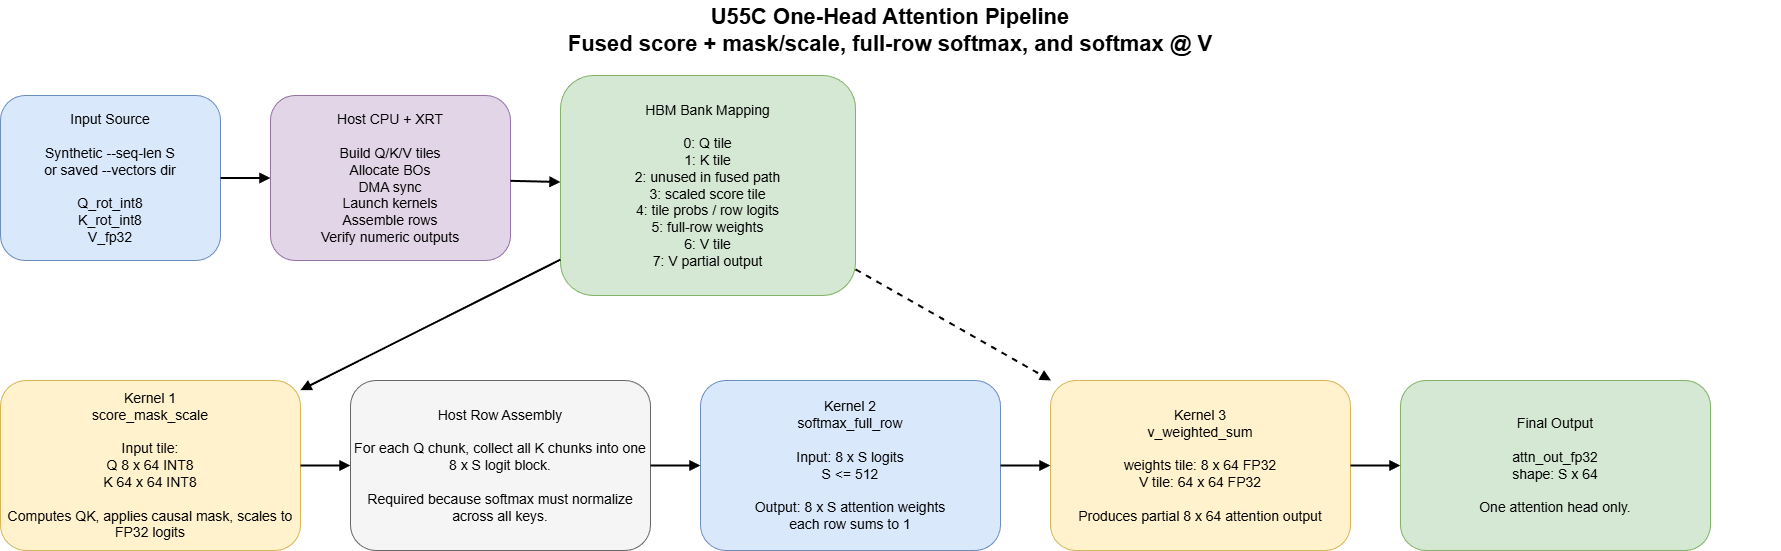
\includegraphics[width=0.92\textwidth]{report_assets/attention_architecture.png}
    \caption{Final one-head attention architecture. The verified design uses
    host/XRT orchestration, HBM banked buffers, fused score-mask-scale,
    full-row softmax, and a value weighted-sum stage.}
    \label{fig:architecture}
\end{figure*}

\subsection{Design Evolution}

Development proceeded through four phases, separating correctness, data
sourcing, and measurement work.

Track A focused on making the score path usable at realistic sequence lengths.
The initial implementation demonstrated a single attention-score tile. That was
useful for validating the arithmetic, but it did not handle full \(S\times S\)
attention. Track A added full-sequence tiling in the Python reference and in
the host application. It also exposed the important softmax issue: for multiple
K chunks, softmax must normalize across the full row, not within each tile. The
full-row softmax kernel was therefore added before long-sequence correctness
could be claimed. Track A also introduced host-side double buffering in the
first pass and eventually fused score, causal mask, and scale into one kernel.

Track B extended the output contract. Before Track B, the FPGA could verify
attention weights, but the attention block in a transformer does not stop at
weights. It multiplies those weights by V to produce the attended output. Track
B added the Python reference for \(PV\), implemented the HLS
value weighted-sum kernel, updated host integration, and changed verification
so that final \(S\times64\) attention output is checked. This made the FPGA
demo much closer to a real transformer attention sub-block.

Track C replaced purely synthetic data with TinyLlama-derived vectors. This
track first verified that the local Python environment could load TinyLlama,
then extracted Q, K, and V tensors from one attention layer, applied the
head-mapping needed for grouped-query attention, quantized Q and K, and exported
saved-vector directories. Track C is the reason this work can claim
TinyLlama-derived input validation rather than only deterministic toy data.

Track D created the measurement story. It added CPU and GPU baselines, real U55C
timing sweeps, utilization reports, and a discussion of what the results do and
do not mean. Track D provides the measurements needed to assess the design against measured software baselines. The FPGA is functionally correct, but the first staged
architecture is not yet faster than the one-head CPU baseline, which motivates the architectural improvements described in the results.

\section{Methodology}

\subsection{Reference Model and Vector Export}

The software reference is written in Python and serves three purposes: it
defines the expected numerical result for each pipeline stage, exports
deterministic synthetic vectors for repeatable unit tests and hardware runs,
and extracts TinyLlama-derived Q/K/V vectors for saved-vector verification.

The synthetic path generates deterministic Q, K, and V tensors for sequence
lengths \(S=8,64,128,256,512\). The Python reference computes raw INT32 scores,
masked and scaled logits, full-row softmax probabilities, and final attention
output. The TinyLlama path loads
\texttt{TinyLlama/TinyLlama-1.1B-Chat-v1.0}, captures Q/K/V at a selected
attention layer, applies the same grouped-query head mapping used by the model,
quantizes Q and K, and writes vector directories under \texttt{sim/}. The
verified real-vector directories include a legacy single-tile case and
full-sequence \(S=16,64,128,256,512\) cases.

The reference scripts intentionally produce simple text files rather than a
binary-only format. This made the files usable by Python, local C++ testbenches,
HLS C simulation, and the XRT host application. The main exported tensors are
Q, K, scaled logits, softmax probabilities, V, and final attention output. The
single-tile directories also preserve raw and masked score references for
debugging. In the fused hardware path, raw scores are internal to the kernel
and are no longer written back to HBM, but keeping the raw-score reference
helped validate that fusion did not change the mathematical contract.

The TinyLlama extraction flow had two checks. First, the setup script loaded the
tokenizer and model and ran a short forward pass to confirm that the software
environment could execute TinyLlama. Second, the Q/K/V extraction script
registered a pre-hook on a selected attention layer, mirrored the model's
projection and RoPE behavior, and compared the selected-head attention result
against PyTorch scaled-dot-product attention. The default extraction run
reported an SDPA maximum difference of approximately \(3.7\times10^{-9}\),
which gave confidence that the saved vectors represented the intended model
subgraph before quantization.

After extraction, Q and K were quantized per tensor. A representative run
reported Q scale \(4.8984\times10^{-2}\), K scale
\(1.7432\times10^{-2}\), Q reconstruction maximum error \(2.45\times10^{-2}\),
K reconstruction maximum error \(8.71\times10^{-3}\), and dequantized score
maximum error \(2.66\times10^{-2}\). These numbers are not model accuracy
measurements; they only quantify the local numerical error introduced by the
INT8 Q/K representation used for this one-head accelerator.

\subsection{HLS Kernel Design}

The verified fused design contains four main kernels in the real-card attention
path:
\begin{enumerate}
    \item \texttt{score\_mask\_scale\_u55c\_kernel}: reads packed INT8 Q and K
    tiles, computes \(QK^T\), applies causal mask and scale, and writes FP32
    logits directly.
    \item \texttt{softmax\_full\_row\_u55c\_kernel}: normalizes up to eight
    full query rows over \(S \leq 512\) keys.
    \item \texttt{softmax\_u55c\_kernel}: preserved for the legacy single-tile
    softmax path.
    \item \texttt{v\_weighted\_sum\_u55c\_kernel}: computes one partial
    \(8\times64\) contribution of \(PV\) from an \(8\times64\) probability tile
    and a \(64\times64\) V tile.
\end{enumerate}

The fused score-mask-scale kernel replaces the earlier staged score GEMM plus
mask/scale kernels. This removes a raw-score HBM round trip and one kernel
launch in the pre-softmax path. The V weighted-sum kernel remains staged:
for each Q chunk, the host launches it once per K/V chunk and accumulates
partial outputs into final \(S\times64\) attention output.

The design history is useful for understanding the final architecture. The
earliest score kernel used a narrow external memory interface and spent most of
its estimated latency loading K. Widening Q, K, and score traffic to packed
64-bit words reduced the score-kernel latency estimate from roughly 5153 cycles
to roughly 1312 cycles. This showed that the first bottleneck was not only the
number of multiply-accumulate operations, but also how data was presented to the
kernel. Later, causal mask and score scale were merged so the design no longer
needed two separate post-score kernels. Finally, score generation, masking, and
scaling were fused into \texttt{score\_mask\_scale\_u55c\_kernel}, which writes
FP32 logits directly.

The full-row softmax kernel was added after the design moved beyond
single-tile sequence lengths. A tile-local softmax is correct only when all
valid keys fit inside one \(8\times64\) tile. For \(S>64\), normalizing each
tile independently would make each tile row sum to one and would over-count
probability mass across K chunks. The full-row kernel therefore accepts an
\(8\times S\) logit block and performs a stable row-wise softmax across all
keys. The current maximum supported full-row length is \(S=512\), matching the
synthetic sweep used for evaluation.

The HLS design uses loop pipelining, unrolling, and array partitioning rather
than a hand-written systolic array. The dot-product loops are unrolled to expose
parallel multipliers, local arrays are partitioned so the pipeline has enough
read ports, and memory interfaces are mapped to HBM banks through the Vitis
link configuration.

The implemented kernels rely on HLS scheduling: data is loaded into local
arrays, loops are pipelined, and selected inner loops are unrolled so multiple
multiply-accumulate operations occur in parallel. This approach is practical to
iterate in C++ HLS and sufficient for the first verified design, but it leaves
room for future hand-optimized or more deeply streaming architectures.

\subsection{XRT Host Flow and HBM Mapping}

The host application is written with the XRT C++ API. It loads the xclbin,
creates kernels, allocates buffer objects, writes vectors, synchronizes buffers
to the device, launches kernels, waits for completion, synchronizes results
back, and compares outputs against reference tensors. The main XRT calls are
\texttt{xrt::device}, \texttt{device.load\_xclbin}, \texttt{xrt::kernel},
\texttt{xrt::bo}, \texttt{bo.write}, \texttt{bo.sync}, kernel invocation,
\texttt{run.wait}, and \texttt{bo.read}.

Table~\ref{tab:hbm} lists the fused design's HBM bank mapping. The earlier raw
score bank is no longer used by the fused pre-softmax path because raw scores
are immediately masked and scaled inside the fused kernel.

The host is also responsible for sequencing dependencies between kernels. For
each Q chunk, it launches the fused pre-softmax kernel across K chunks, gathers
the resulting \(8\times64\) logit tiles into an \(8\times S\) row block,
launches full-row softmax, slices the probabilities back into K-sized blocks,
launches V weighted-sum kernels, and accumulates the partial \(8\times64\)
outputs. This makes the data flow easy to verify because every major
intermediate is visible to the host. It also explains why the final design has
substantial overhead: the host remains in the middle of the attention data path.

\begin{table}[t]
\centering
\caption{HBM bank mapping in the fused verified path.}
\label{tab:hbm}
\begin{tabular}{ll}
\toprule
Data buffer & HBM bank \\
\midrule
Q tile & HBM[0] \\
K tile & HBM[1] \\
Fused scaled logits & HBM[3] \\
Tile probability / full-row logits & HBM[4] \\
Full-row probability / V weights & HBM[5] \\
V chunk & HBM[6] \\
V partial output & HBM[7] \\
\bottomrule
\end{tabular}
\end{table}

\subsection{Verification Flow}

Verification was performed in layers. Python reference checks validated the
math for full-sequence tiling at \(S=8,64,128,256,512\). Local C++ testbenches
validated individual HLS kernels against exported files. Vitis HLS C simulation
and synthesis were run for the kernel implementations. XRT hardware emulation
validated the compiled xclbin and host application before running on the real
card. Finally, the hardware bitstream was executed on a U55C and compared
against software references.

This work did not use Vitis HLS C/RTL co-simulation. Instead, the verification
chain combined Python references, local C++ tests, HLS \texttt{csim},
\texttt{csynth}, XRT \texttt{hw\_emu}, and real-card XRT execution. The
expected pass signal for full attention runs is:
\[
\texttt{Attention output verification PASSED}
\]
followed by:
\[
\texttt{XRT chain verification PASSED}.
\]
Floating-point comparisons use a tolerance of \(10^{-4}\) for most synthetic
and intermediate comparisons, with a larger \(10^{-3}\) tolerance for some
TinyLlama-derived final attention outputs where quantization and PyTorch
reference differences are larger.

The verification flow deliberately separates correctness from performance. A
kernel can pass HLS simulation and still fail to place, route, or perform well
after integration. Conversely, hardware emulation can validate API-level
behavior and final output, but its runtime is simulator dominated and should not
be used as a performance estimate. Real-card timing is therefore reported only
from U55C hardware runs with \texttt{XCL\_EMULATION\_MODE} unset.

\subsection{Experimental Setup}

The FPGA experiments used Vitis/Vivado 2022.2, XRT 2022.2, and the U55C
platform \texttt{xilinx\_u55c\_gen3x16\_xdma\_3\_202210\_1}. The card shell
reported \texttt{xilinx\_u55c\_gen3x16\_xdma\_base\_3}. The real-card runs used
device index 0. Hardware builds produced an xclbin bitstream, which the host
loaded through XRT. Table~\ref{tab:platform} summarizes the platform and
software environment.

\begin{table}[t]
\centering
\caption{FPGA platform and software environment.}
\label{tab:platform}
\begin{tabular}{ll}
\toprule
Component & Details \\
\midrule
FPGA card & AMD/Xilinx Alveo U55C \\
FPGA device & \texttt{xcu55c-fsvh2892-2L-e} \\
Platform & \texttt{xilinx\_u55c\_gen3x16\_xdma\_3\_202210\_1} \\
Tools & Vitis/Vivado/Vitis HLS 2022.2 \\
Runtime & XRT 2022.2 \\
Host compiler & \texttt{g++} with C++17 \\
Kernel clock & 300 MHz target \\
HBM clock & 450 MHz \\
\bottomrule
\end{tabular}
\end{table}

CPU baselines were measured with the repository's NumPy/Python benchmark
scripts. GPU baselines were measured separately on a Windows laptop with
PyTorch 2.11.0+cu128, CUDA 12.8, and an NVIDIA GeForce RTX 3050 Laptop GPU. The
GPU baseline is useful as a PyTorch comparison point, but it is not a
same-host measurement with the Linux/U55C system. This distinction is important
when interpreting speedup tables.

The FPGA hardware build produces multiple artifacts beyond the host executable.
The checked-in report set includes xclbin information, link summaries, system
diagrams, routed timing summaries, full-design utilization, per-kernel
utilization, and SLR utilization. These artifacts support the timing-closure
and resource claims in the Results section.

\section{Results and Discussion}

\subsection{Functional Verification}

Table~\ref{tab:verification} summarizes the main verification outcomes. The
final fused design was validated with both synthetic inputs and saved
TinyLlama-derived vectors. Synthetic sequence lengths cover multiple tile
shapes, including multi-K-chunk cases. Real TinyLlama saved-vector directories
currently cover \(S=16,64,128,256,512\), plus the legacy single-tile case.

\begin{table}[t]
\centering
\caption{Verification summary for the fused one-head attention path.}
\label{tab:verification}
\begin{tabular}{p{0.31\linewidth}p{0.55\linewidth}}
\toprule
Stage & Result \\
\midrule
Python reference & Full tiling check passed for \(S=8,64,128,256,512\). \\
Local C++ benches & Score, fused score-mask-scale, softmax, full-row softmax,
and V weighted sum passed. \\
Vitis HLS & Relevant kernels passed \texttt{csim} and \texttt{csynth}. \\
XRT \texttt{hw\_emu} & Fused vector and sequence tests passed. \\
Real U55C & Synthetic \(S=8,64,128,256,512\) and real-vector
\(S=16,64,128,256,512\) passed through final attention output. \\
\bottomrule
\end{tabular}
\end{table}

The most important functional result is that the FPGA output is verified at the
final attention-output tensor, not only at intermediate scores. Earlier stages
of this work verified attention weights, but Track B extended the design so
that \(PV\) is also computed and checked. This makes the result
more representative of the actual attention block used by a transformer layer.
At the same time, the output remains one-head \(S\times64\) data, not generated
text or model logits over the vocabulary.

\subsection{Latency Results}

Table~\ref{tab:synthetic} shows synthetic timing results. The staged FPGA
baseline uses separate pre-softmax stages, while the fused FPGA design combines
score computation, masking, and scaling. The fused path improves all synthetic
sequence lengths relative to the staged FPGA baseline, with a 1.21x improvement
at \(S=512\). However, the FPGA remains slower than the CPU and GPU baselines
for this isolated one-head workload.

\begin{table*}[t]
\centering
\caption{Synthetic one-head attention latency. Lower is better. The final
column is CPU time divided by fused FPGA time; values below 1 mean the FPGA is
slower than CPU.}
\label{tab:synthetic}
\begin{tabular}{rrrrrrrr}
\toprule
\(S\) & Tiles & CPU ms & GPU ms & Staged FPGA ms & Fused FPGA ms & Fused/Staged & FPGA speedup vs CPU \\
\midrule
8   & 1   & 0.0322 & 0.3349 & 0.803  & 0.296  & 2.71x & 0.11x \\
64  & 8   & 0.2920 & 0.2507 & 2.864  & 2.364  & 1.21x & 0.12x \\
128 & 32  & 2.5009 & 0.2998 & 6.992  & 5.484  & 1.28x & 0.46x \\
256 & 128 & 3.9523 & 0.2726 & 20.570 & 17.307 & 1.19x & 0.23x \\
512 & 512 & 12.3290 & 0.2461 & 72.941 & 60.328 & 1.21x & 0.20x \\
\bottomrule
\end{tabular}
\end{table*}

Table~\ref{tab:realvectors} shows real TinyLlama-derived saved-vector results.
The fused design improves the full-sequence \(S=16\) and \(S=64\) real-vector
runs compared with the staged FPGA baseline. The legacy single-tile
\texttt{real\_tinyllama\_tile} case is slower after fusion, which is treated as
a small-run overhead/noise case rather than the representative regime. The
larger real-vector \(S=128\), \(S=256\), and \(S=512\) directories were
generated with CUDA/FP16 from the cached TinyLlama model, CPU-sanity checked
locally, and then timed and verified on the real U55C.

\begin{table}[t]
\centering
\caption{Real TinyLlama saved-vector latency.}
\label{tab:realvectors}
\begin{tabular}{lrrrr}
\toprule
Case & \(S\) & CPU ms & Staged ms & Fused ms \\
\midrule
\texttt{real\_tinyllama\_tile} & tile & n/a & 0.258 & 0.635 \\
\texttt{real\_tinyllama\_s16} & 16 & 0.0426 & 1.488 & 0.569 \\
\texttt{real\_tinyllama\_s64} & 64 & 0.1523 & 3.094 & 2.004 \\
\texttt{real\_tinyllama\_s128} & 128 & n/a & n/a & 6.816 \\
\texttt{real\_tinyllama\_s256} & 256 & n/a & n/a & 17.192 \\
\texttt{real\_tinyllama\_s512} & 512 & n/a & n/a & 55.329 \\
\bottomrule
\end{tabular}
\end{table}

The new larger real-vector directories have no staged FPGA, CPU, or GPU timing
entries in the table because they were added after the main staged comparison
run. Their purpose is to strengthen real-input coverage of the fused U55C path.
Local CPU sanity checks reported zero tiled-versus-brute differences for both
softmax probabilities and final \texttt{attn\_out}, with exported softmax-file
maximum difference \(2.98\times10^{-8}\). During the first U55C run,
\texttt{real\_tinyllama\_s128} exposed a verifier-only issue in masked scaled
logits: values around \(-114388\) differed by \(0.0078125\), which exceeded the
old fixed \(10^{-4}\) absolute tolerance but was only about \(6.8\times10^{-8}\)
relative error. The host verifier now allows a conservative \(10^{-6}\)
relative tolerance for scaled-logit comparisons while keeping softmax and
attention-output checks on their existing absolute tolerances.
Synthetic and real-vector timings were collected in separate hardware runs, so
small differences at the same sequence length are interpreted as run-to-run
host, XRT, and card variability rather than a systematic data-content effect.

The synthetic sweep shows that total FPGA latency grows with sequence length,
as expected from the \(S^2\) score matrix and the increasing number of tile
launches. The fused path is consistently better than the staged FPGA baseline
for synthetic tests because the pre-softmax chain is shorter. However, the FPGA
speedup over CPU remains below 1.0 for every tested sequence length, meaning
the CPU baseline is faster for this isolated workload. The higher ratio at
\(S=128\) is reported as measured and is
interpreted as CPU baseline variability for this small one-head benchmark
rather than a change in FPGA scaling, since FPGA launch count still grows with
tile count. At \(S=512\), the FPGA would need roughly a 5x end-to-end
improvement to beat the measured CPU baseline. That level of improvement is
unlikely to come from small HLS pragma tuning alone.

The measured GPU times are nearly flat across the synthetic sequence lengths in
the table. This is partly because the benchmarked one-head problem is small
relative to the GPU's available compute and library overheads. The GPU is not
being saturated in the same way it would be for a full model or batched
workload. The GPU is substantially faster for these small, dense operations because
PyTorch/CUDA launch overhead is small relative to the compute work.

The comparison also highlights why the evaluation scope must be stated
carefully. A full TinyLlama layer would compute all heads, apply output
projection, and continue through the rest of the decoder block. The reported
tables isolate only one attention head after Q/K/V are already prepared. This
is the right scope for testing the FPGA attention block, but it is not a claim
about complete model latency. In a complete accelerator, some fixed host
overheads could be amortized across more heads or fused with neighboring model
operations; the present staged design does not yet do that.

\subsection{Utilization and Timing Closure}

The final routed fused xclbin closes timing on the U55C. The post-route timing
summary reports WNS \(=0.003\) ns, TNS \(=0\), WHS \(=0.009\) ns, and no failing
setup or hold endpoints. The HLS kernels target approximately 300 MHz, and the
platform reports HBM at 450 MHz.

Table~\ref{tab:util} summarizes post-route utilization. The full routed design,
including the platform, uses 14.70\% CLB LUTs, 9.72\% CLB registers, 15.35\%
Block RAM tiles, 0.21\% URAM, and 4.53\% DSP. The user kernels are therefore
not capacity-limited in the fused baseline. The largest kernel is
\texttt{v\_weighted\_sum\_u55c\_kernel}, which uses 320 DSP and dominates the
user-kernel DSP count.

\begin{table}[t]
\centering
\caption{Routed utilization for the fused score-mask-scale xclbin.}
\label{tab:util}
\begin{tabular}{lrrr}
\toprule
Resource & Used & Available & Util. \\
\midrule
CLB LUTs & 191,648 & 1,303,680 & 14.70\% \\
CLB registers & 253,388 & 2,607,360 & 9.72\% \\
BRAM tiles & 309.5 & 2,016 & 15.35\% \\
URAM & 2 & 960 & 0.21\% \\
DSP & 409 & 9,024 & 4.53\% \\
\bottomrule
\end{tabular}
\end{table}

Figure~\ref{fig:utilization} shows the same routed utilization profile
visually.

\begin{figure}[t]
    \centering
    
\includegraphics[width=\linewidth]{report_assets/post_route_utilization.png}
    \caption{Post-route utilization for the fused design. Resource usage is
    modest across all categories, indicating that the performance bottleneck
    is orchestration overhead rather than compute capacity.}
    \label{fig:utilization}
\end{figure}

The utilization numbers show that the fused baseline is not close to filling
the FPGA. This is encouraging for future parallelization, because additional
compute units or a more integrated online-attention kernel may fit. It also
means that the current poor speedup is not due to lack of raw FPGA resources.
Instead, the problem is that the resources are not kept busy enough. The host
must repeatedly launch small kernels and synchronize buffers, so the data path
has idle time between useful compute regions.

The V weighted-sum kernel is the largest individual kernel in the verified
baseline. It consumes 320 DSP, while the fused score-mask-scale kernel consumes
67 DSP and the softmax kernels are much smaller. This aligns with the
mathematics: after softmax, each \(8\times64\) probability tile is multiplied
by a \(64\times64\) V tile, producing 512 output elements through many
floating-point multiply-accumulate operations. Future designs must either make
this stage more resident and less host-driven or fuse it with online softmax so
the probability matrix is never staged as a separate full tensor.

SLR utilization is also useful for interpreting future designs. The verified
fused baseline closes timing and uses a modest fraction of the full device, but
larger experimental kernels can still fail if their placement is concentrated
in one region or creates too many routing/control-set constraints. Therefore,
future optimization work should not look only at total DSP percentage. It must
also consider pblock capacity, SLR placement, routing pressure, and whether the
datapath is too wide to route cleanly at the target clock.

\subsection{Discussion of Bottlenecks}

The primary lesson from the results is that kernel correctness and timing
closure are not sufficient for end-to-end acceleration. At \(S=512\), the fused design still issues 512 score-mask-scale launches,
64 softmax launches, and 512 V launches --- 1088 total.
The host also assembles full rows, slices probability tiles, moves V chunks,
and accumulates partial outputs. The U55C has substantial remaining resources,
but the current orchestration exposes too much intermediate state to
host-visible buffers and pays many launch/synchronization costs.

Score-mask-scale fusion helps because it removes one kernel launch and one
raw-score HBM round trip from the pre-softmax path. It does not address the deeper issue that
softmax and value accumulation remain separate staged passes. This explains why
the fused design improves FPGA-to-FPGA comparisons but still does not beat the
CPU baseline for the isolated one-head workload.

The GPU baseline is especially fast for these small cases because PyTorch and
CUDA execute the matrix operations with highly optimized libraries and low
effective launch overhead relative to the work. The CPU baseline is also strong
because the one-head matrices are small enough to fit comfortably in cache. A
more favorable FPGA comparison would require either more parallel heads, larger
batches, longer sequences, or a more integrated FPGA-native attention kernel
that keeps the full computation on card.

Another bottleneck is that the current design does not use all available HBM
parallelism. It maps logical buffers across several banks, which prevents all
traffic from contending for one memory channel, but it does not fully exploit
the 32 HBM pseudo-channels available on the U55C. The buffer sizes in the
verified one-head tests are also small compared with total HBM capacity. Thus,
the design is not capacity-limited; it is limited by orchestration, launch
granularity, and the amount of data staged between kernels.

The current design also accelerates only one selected head. TinyLlama has 32
query heads and 4 key/value heads. In the real model, multiple heads are
computed as part of the same layer. An FPGA design that processes several heads
or several Q chunks concurrently could use more DSPs and HBM bandwidth and
would provide a more realistic throughput comparison. This work stops before
that scale-out step so the one-head path can be verified carefully first.

\subsection{Optimization Direction}

Three architectural improvements are needed before minor clock tuning becomes
relevant. First, full Q/K/V and intermediate
buffers should remain resident on device so the host reads back only final
attention output during normal operation. Second, launch count should be
reduced by using larger-grain kernels that process all K chunks for one Q
chunk. Third, online softmax should be fused with value accumulation so the
design no longer materializes the full \(S\times S\) probability matrix. In
online softmax, each query row maintains a running maximum, exponential sum,
and \(64\)-element value accumulator while streaming through K/V chunks. This
would replace the current logit-materialization, full-row softmax, probability
staging, and V weighted-sum sequence with a single attention-output-producing
kernel per Q chunk.

The expected optimization path is incremental. A device-resident flow should
first copy Q, K, and V to device memory once and read back only final attention
output in the normal path. A launch-count reduction should then move from
per-tile launches to one pre-softmax and one value-accumulation launch per Q
chunk. Finally, online softmax should remove the need to store a full
\(S\times S\) probability matrix. Each step is validated against the same output references so correctness is
not lost as performance improves.

\subsection{Limitations}

The design is not full TinyLlama inference and does not report model-level
tokens per second. The
real TinyLlama saved-vector coverage now reaches \(S=512\), but it is still
limited to one selected layer/head and saved prompt vectors rather than live
decoder integration. The larger \(S=128,256,512\) real-vector cases also do not
yet have staged FPGA, CPU, or GPU timing baselines in the results table. The GPU
baseline was measured on a separate laptop rather than the U55C host machine.
Finally, the FPGA implementation uses FP32 for softmax and V accumulation,
which simplifies verification but is not necessarily the final numeric format
for a production accelerator.

Another limitation is that the design does not yet use a KV-cache-aware decode
path. This matters because LLM inference has two phases. During prompt prefill,
many query rows are processed together. During decode, each generated token
usually introduces one new query row that attends over cached keys and values.
The current full-sequence saved-vector tests are closer to prefill validation.
A deployed edge LLM accelerator would need a cache layout, update policy, and
decode-time host or controller interface. Those pieces are outside the verified
scope but are natural extensions once the attention kernel itself is more
integrated.

\section{Conclusion}

This work implemented and verified an isolated one-head transformer attention
block on a Xilinx Alveo U55C FPGA. The final fused design computes
INT8 query-key scores, applies causal masking and dequantization scaling,
performs full-row softmax, and computes \(\mathrm{softmax}(QK^T)V\) to produce
FP32 one-head attention output. The design is verified through local reference
checks, HLS simulation and synthesis, hardware emulation, and real U55C
execution. Synthetic sequences up to \(S=512\) and TinyLlama-derived saved
vectors at \(S=16,64,128,256,512\) pass final output verification.

The FPGA implementation is correct and timing-clean, but it is not faster than
the CPU or GPU baselines for this isolated one-head workload. The fused pre-softmax kernel improves the
staged FPGA baseline, yet the design remains dominated by many small kernel
launches and HBM-visible intermediate transfers. The design is best understood as a validated hardware baseline and design
study rather than a final high-performance LLM accelerator. The next step is to make the computation more
FPGA-native by keeping buffers resident, reducing launch count, fusing online
softmax with V accumulation, and eventually scaling across multiple Q blocks or
attention heads.

\begin{thebibliography}{9}

\bibitem{nielsen2015neural}
M. A. Nielsen, \emph{Neural Networks and Deep Learning}. Determination Press,
2015. [Online]. Available: \url{http://neuralnetworksanddeeplearning.com/}

\bibitem{alammar2018illustrated}
J. Alammar, ``The illustrated transformer,'' 2018. [Online]. Available:
\url{https://jalammar.github.io/illustrated-transformer/}

\bibitem{leo2024math}
C. Leo, ``The math behind transformers,'' \emph{Medium}, accessed 2026.
[Online]. Available:
\url{https://medium.com/@cristianleo120/the-math-behind-transformers-6d7710682a1f}

\end{thebibliography}

\section{Student Contributions}

\textbf{Om Girish Sheladia} designed and implemented Track~A Steps~1 and~2. This included the
16-way unrolled INT8 score GEMM work, 64-bit packed memory I/O for the score
path, and the fused causal-mask and score-scale kernel that removed an
intermediate HBM round trip. Om also ran HLS synthesis and helped verify the
early optimized score path on U55C hardware.

\textbf{Samarth Bangalore Sudharshan} designed and implemented Track~A Steps~3 through~5. This
included the Python full-sequence tiling reference, full-row softmax support for
\(S\leq512\), the XRT host tiling loop, pre-softmax host double buffering, and the
fused score-mask-scale kernel used in the final verified design. Samarth also
verified tiled synthetic runs on the real U55C for \(S=8,64,128,256,512\).

\textbf{Rijul Wankhade} designed and implemented Track~B. Rijul added the
\texttt{v\_weighted\_sum} HLS kernel for the \(PV\) stage,
integrated it into the host flow as the value-accumulation pass, and changed
verification so the FPGA checks final one-head \texttt{attn\_out} rather than
only attention weights. This completed the one-head attention output path.

\textbf{Satyarth Guna Motupalli} implemented Track~C and Track~D. This included TinyLlama Q/K/V
extraction through a PyTorch forward hook, INT8 symmetric quantization for Q and
K, full-sequence real-vector export through \(S=512\), CPU and GPU baseline
benchmarks, and the performance comparison tables and analysis used in this
report. Satyarth also verified the complete path with real TinyLlama-derived
vectors on the U55C.

\end{document}
